\documentclass[10pt]{article}
\usepackage[margin=0.82in]{geometry}
\usepackage[T1]{fontenc}
\usepackage{lmodern}
\usepackage{amsmath,amssymb,amsthm}
\usepackage{graphicx}
\usepackage{microtype}
\usepackage[hidelinks]{hyperref}
\usepackage{enumitem}
\usepackage{float}

\newtheorem*{theorem}{Theorem}
\newtheorem*{lemma}{Confluence lemma}
\newcommand{\A}{\mathcal A(\mathbb D)}
\newcommand{\D}{\mathbb D}
\newcommand{\spn}{\operatorname{span}}

\begin{document}

\begin{center}
{\Large No cumulative finite-Blaschke basis of the disk algebra}\\[3pt]
{\large A literature-implied full answer to Question 7.4 of arXiv:2507.13121}
\end{center}

\paragraph{Status.}
\textbf{Literature-implied full negative answer.}
The decisive obstruction is Theorem~4 of Ivanov--Shekhtman (2001), which
predates the source question.  The reduction below includes repeated zeros,
which ordinary point interpolation does not cover verbatim.

\paragraph{Source and exact question.}
The source is E. Fricain, J. Mashreghi, M. Nasri, and M. Ostermann,
\emph{Schauder Basis with Finite Blaschke Products}, arXiv:2507.13121v2.
It sets
\[
 B_0=1,\qquad
 B_n(z)=\prod_{k=1}^n b_{\lambda_k}(z),\qquad
 b_\lambda(z)=\frac{\lambda-z}{1-\overline\lambda z},
\]
and calls $(\lambda_n)$ non-Blaschke when
$\sum_n(1-|\lambda_n|)=\infty$.

\begin{figure}[H]
\centering
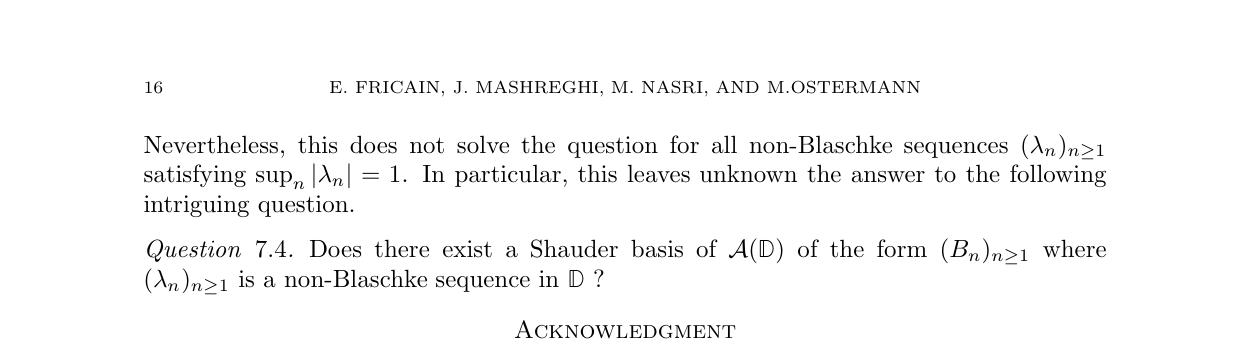
\includegraphics[width=.95\textwidth]{figures/question_7_4_crop.png}
\caption{Question 7.4 on printed page 16 of arXiv:2507.13121v2.}
\end{figure}

The displayed indexing starts at $1$.  Literally, that version has the
immediate negative answer: every $B_n$, $n\ge1$, vanishes at $\lambda_1$, so
its closed span is contained in the proper ideal
$\{f\in\A:f(\lambda_1)=0\}$.  We prove the stronger intended statement for
the complete family $(B_n)_{n\ge0}$.

\paragraph{Idea of proof.}
The tail of the proposed basis is not an arbitrary subspace: after the first
$N$ terms it is exactly the principal ideal $B_N\A$.  Thus the $N$th basis
projection is the Hermite interpolation projection at the zeros of $B_N$,
counted with multiplicity.  Split repeated nodes into nearby distinct nodes.
The associated Lagrange projections converge in operator norm to the Hermite
projection.  A putative basis would therefore yield point-interpolation
projections converging to the identity, which Ivanov--Shekhtman proved
impossible in the disk algebra.

\begin{theorem}
For every non-Blaschke sequence $(\lambda_n)\subset\D$, repetitions allowed,
the cumulative family $(B_n)_{n\ge0}$ is not a Schauder basis of $\A$.
Consequently Question 7.4 has a negative answer under either its literal or
its intended indexing.
\end{theorem}

\begin{proof}
Assume that $(B_n)_{n\ge0}$ is a Schauder basis of $\A$, and let
\[
 S_N\!\left(\sum_{n\ge0}a_nB_n\right)=\sum_{n=0}^{N-1}a_nB_n,
 \qquad E_N=\spn\{B_0,\ldots,B_{N-1}\}.
\]
Then $S_Nf\to f$ for every $f\in\A$ and
\[
 \ker S_N=\overline{\spn}\{B_n:n\ge N\}.
\]
Write $B_{N+k}=B_NC_k$, where $C_0=1$ and $C_k$ is the cumulative product
formed from $\lambda_{N+1},\ldots,\lambda_{N+k}$.  Removing finitely many
terms preserves the non-Blaschke condition.  The source paper's completeness
criterion therefore gives
$\overline{\spn}\{C_k:k\ge0\}=\A$.  Multiplication by $B_N$ is an isometry
of $\A$ onto the closed ideal $B_N\A$, since $|B_N|=1$ on $\partial\D$.
Hence
\begin{equation}\label{eq:kernel}
 \ker S_N=B_N\A.
\end{equation}

Let $\alpha_1,\ldots,\alpha_s$ be the distinct zeros of $B_N$, with
multiplicities $m_1,\ldots,m_s$; thus $\sum_jm_j=N$.  Divisibility by $B_N$
is equivalent to vanishing of the jets
\[
 f^{(r)}(\alpha_j),\qquad 1\le j\le s,\quad 0\le r<m_j.
\]
Equation~\eqref{eq:kernel} says precisely that $S_Nf$ is the unique element of
$E_N$ sharing all these jets with $f$.  (Uniqueness also follows from
$E_N\cap B_N\A=\{0\}$.)  Thus $S_N$ is a confluent, or Hermite,
interpolation projection.

For this fixed $N$, replace the $m_j$ copies of each $\alpha_j$ by $m_j$
distinct points $\alpha_{j,r}(t)\in\D$ tending to $\alpha_j$ as $t\downarrow0$.
For all sufficiently small $t$, interpolation at the resulting $N$ distinct
nodes is unisolvent on $E_N$; denote its projection by $L_{N,t}:\A\to E_N$.
The confluence lemma below gives
\begin{equation}\label{eq:confluence}
 \|L_{N,t}-S_N\|_{\A\to\A}\longrightarrow0.
\end{equation}
Choose $t_N$ so small that the norm in \eqref{eq:confluence} is less than
$1/N$, and put $L_N=L_{N,t_N}$.  Each $L_N$ is a projection determined only
by the values of its input on a finite set $Z_N\subset\D$.  Moreover, for
every $f\in\A$,
\[
 \|L_Nf-f\|_\infty
 \le \|(L_N-S_N)f\|_\infty+\|S_Nf-f\|_\infty
 \le \frac{\|f\|_\infty}{N}+\|S_Nf-f\|_\infty\longrightarrow0.
\]

This contradicts Ivanov--Shekhtman, Theorem~4: for arbitrary finite sets
$Z_N\subset\D$ and arbitrary projections $L_N$ depending only on values on
$Z_N$, there is an $f\in\A$ for which $L_Nf$ does not converge to $f$.
The assumed Schauder basis cannot exist.
\end{proof}

\begin{lemma}
With the notation above, $L_{N,t}\to S_N$ in operator norm as the distinct
nodes coalesce to the zeros of $B_N$ with their prescribed multiplicities.
\end{lemma}

\begin{proof}
Let $V_t:\A\to\mathbb C^N$ be the value map at the split nodes.  Within each
cluster apply the standard Newton divided-difference change of coordinates
$D_t$ to $V_t$.  Because all limiting nodes lie strictly inside $\D$, Cauchy
estimates on fixed small disks show, uniformly for $\|f\|_\infty\le1$, that
$D_tV_tf$ converges to the jet vector
\[
 Jf=\bigl(f^{(r)}(\alpha_j)/r!\bigr)_{j,r}.
\]
The same convergence holds for the restrictions to the fixed
finite-dimensional space $E_N$.  The restriction $J|_{E_N}$ is invertible,
since its kernel is $E_N\cap B_N\A=\{0\}$.  Consequently
\[
 L_{N,t}
 =\bigl((D_tV_t)|_{E_N}\bigr)^{-1}D_tV_t
 \longrightarrow (J|_{E_N})^{-1}J=S_N
\]
in operator norm, by continuity of inversion in finite dimensions.
\end{proof}

\paragraph{Literature and novelty scope.}
For pairwise distinct $\lambda_n$, the contradiction is essentially immediate
from the 2001 theorem: $S_Nf$ interpolates $f$ at
$\lambda_1,\ldots,\lambda_N$.  The confluence argument closes the repetition
case allowed by the source definition.  The run therefore records this as a
literature-implied answer, not as a new independent solution.  A bounded
search through 2026-08-11 found no later paper needed for the conclusion.

\paragraph{Review recommendation.}
The mathematical reduction is short and checkable, but the status should
remain \emph{literature-implied}: verify the cited formulation of
Ivanov--Shekhtman Theorem~4, then notify the source authors of the pre-existing
interpolating-basis obstruction and the confluent-node extension.

\begin{thebibliography}{9}
\bibitem{source}
E. Fricain, J. Mashreghi, M. Nasri, and M. Ostermann,
\emph{Schauder Basis with Finite Blaschke Products},
arXiv:2507.13121v2 (2026).

\bibitem{IS}
I. V. Ivanov and B. Shekhtman,
\emph{Linear discrete operators on the disk algebra},
Proc. Amer. Math. Soc. \textbf{129} (2001), 1987--1993,
\href{https://doi.org/10.1090/S0002-9939-00-05774-9}{doi:10.1090/S0002-9939-00-05774-9}.
\end{thebibliography}

\end{document}

